\documentclass[a4paper, 12pt]{report}

\usepackage{amsmath}
\usepackage{esint}
\usepackage{comment}
\usepackage{amssymb}
\usepackage{commath}
\usepackage{geometry}
\usepackage{graphicx}
\usepackage{hyperref}
\usepackage{listings}
\usepackage{xcolor}
\usepackage{array}
\usepackage{longtable}

\definecolor{codegreen}{rgb}{0,0.6,0}
\definecolor{codegray}{rgb}{0.5,0.5,0.5}
\definecolor{codepurple}{rgb}{0.58,0,0.82}
\definecolor{backcolour}{rgb}{0.95,0.95,0.92}

\def\t{\theta}
\def\a{\alpha}
\def\be{\beta}
\def\w{\omega}
\def\la{\lambda}
\def\g{\gamma}
\def\f{\frac}
\def\l{\left}
\def\r{\right}
\def\dst{\displaystyle}
\def\b{\bar}
\def\h{\hat}
\def\ph{\phi}
\def\d{\cdot}
\def\n{\nabla}
\def\p{\partial}
\def\lap{\mathcal{L}}
\def\sizem{0.93}
\def\size{0.39}
\def\tabsize{4.4cm}
\def\stabsize{0.97cm}
\def\mtabsize{0.73cm}
\def\ltabsize{5.5cm}

%\let\stdsection\section
%\renewcommand\section{\newpage\stdsection}
\geometry{portrait, margin= 0.47in}

\begin{document}

\title{Scheduler Variations}
\author{Hans C. Suganda}
\date{$8^{th}$ January 2022}
\maketitle
\newpage

\lstset{
	columns=fullflexible,
	frame=single,
	breaklines=true,
	backgroundcolor=\color{backcolour},   
	commentstyle=\color{codegreen},
	keywordstyle=\color{magenta},
	numberstyle=\tiny\color{codegray},
	stringstyle=\color{codepurple},
	basicstyle=\ttfamily\footnotesize,
	keepspaces=true,                 
	numbersep=5pt,                  
	showspaces=false,               
	showtabs=false,                  
	tabsize=2
}

\tableofcontents
\newpage

\begin{center}
\begin{comment}

For cases exponential, linear piecewise and inverse decay:
    Change the code block in modified helmholtz (done)
    Ensure scheduler works properly (done)
    Populate the data directory with post-processing script (done)
    Fill the NN_WB_Input file (done)
    Figure out how to run on RCAC (done)
    Run and collect Data 

Parameters to test:
    Width:10,30,50 | Depth:1-10
    Width:80,100 | Depth:1-10
    Width:140,200 | Depth:1-8

The actual learning rate in the previous attempts were 1e-04, this is because in the previous attempts, the default learning rate which was 1e-03 was multiplied by 0.1 to form 1e-04 (true learning rate)

Make the initial learning rates perhaps 5e-04 and the resting learning rates for the various scheduler schemes perhaps 3e-05

To connect to Bell:
    connect hsuganda@bell.rcac.purdue.edu

Loading Necessary Modules:
    module load learning/conda-2020.11-py38-cpu
    module load ml-toolkit-cpu/keras

Command to Run:
    nohup sh Case_Input > Case_log.txt &

Declare directories inside Expo, Inv and Poly
Modify Convergence Plot to accept two data files
Copy to Post processing tools

Command for Images:
\begin{figure}[H]\centering\\includegraphics[scale=\sized]{Computational_Domain_Final.jpg}\caption{Computational domain with planes of symmetry}\end{figure}

Chosen Width: 80
Chosen Depth: 5

\end{comment}
%Seperator
%Seperator
%Seperator
%Seperator
%Seperator
\section{Rationale}
\begin{comment}
\end{comment}
Previously, it was established that as the weights of the neural network approached a local minima in the loss function, the learning rate must be reduced in order not to "overshoot" the local minima and cause stability issues. This stability issue seems more prominent in "larger" neural network architectures containing more nodes and hidden layers. Here a learning rate scheduler is implemented which allows the learning rate to change with the number of training iterations. As the number of training iterations increase, the learning rate reduces based on a variety of pre-defined functions. This was implemented in the hopes of accelearting training of the neural network at lower training iterations where stability is not likely to be an issue but then reducing the learning rate when the neural network has been sufficiently trained and stability issues are likely to occur. 
%Seperator
%Seperator
%Seperator
%Seperator
%Seperator
\section{Algorithm Changes}
\begin{comment}
\end{comment}
Generally, only a minor piece of the code must be modified, namely where the learning rate scheduler was defined.
%Seperator
%Seperator
%Seperator
%Seperator
\subsection{Exponential LR}
\begin{comment}
\end{comment}
The initial modification sets the learning rate to exponential decay. The code is shown below,
\begin{lstlisting}[language=python]
#Determine the Learning Rate
lr_schedule = keras.optimizers.schedules.ExponentialDecay(
    initial_learning_rate=5e-4,
    decay_steps=250000,
    decay_rate=0.06,
    name=None)
\end{lstlisting}
%Seperator
%Seperator
%Seperator
%Seperator
\subsection{Polynomial LR}
\begin{comment}
\end{comment}
Another type of scheduling scheme that \url{keras} allows is the polynomial decay. The code is shown below,
\begin{lstlisting}[language=python]
#Determine the Learning Rate
lr_schedule = keras.optimizers.schedules.PolynomialDecay(
    initial_learning_rate=5e-4,
    decay_steps=250000,
    end_learning_rate= 3e-5,
    power=1,
    cycle=False,
    name=None)
\end{lstlisting}

%Seperator
%Seperator
%Seperator
%Seperator
\subsection{Inverse LR}
\begin{comment}
\end{comment}
The last scheme that is used in this short investigation is inverse decay. The code is shown below,
\begin{lstlisting}[language=python]
#Determine the Learning Rate
lr_schedule = keras.optimizers.schedules.InverseTimeDecay(
    initial_learning_rate=5e-4,
    decay_steps=250000,
    decay_rate=15.66666,
    staircase=False,
    name=None)
\end{lstlisting}

%Seperator
%Seperator
%Seperator
%Seperator
%Seperator
\section{Choice of Parameters}
\begin{comment}
\end{comment}
To facilitate a direct comparison to previous results, the number of maximum training iterations here is kept identical to the number of training iterations in the previous work. Therefore, the maximum number of training iterations is $250000$. In this investigation, the learning rate should be somewhat comparable to the previous learning rate. Since the learning rate of the previous work is $1e-4$, the initial learning rate here is chosen to be $5e-4$. The final learning rate after $250000$ training iterations is chosen to be $3e-5$. These choices are somewhat arbitrary, but the decision was made with the idea that the initial learning rate should be higher to facillitate faster convergence but the "final" learning rate should be lower to avoid stability issues.
%Seperator
%Seperator
%Seperator
%Seperator
\subsection{Exponential LR}
\begin{comment}
\end{comment}
The exponential decay learning rate function introduces $3$ main variables. The true learning rate represented as \url{lr} is defined below,
\begin{lstlisting}[language=python]
lr = initial_learning_rate * decay_rate ^ (step / decay_steps)
\end{lstlisting}
The current training iteration number is represented by the variable \url{step}. The exponential decay means that the learning rate will decay by \url{decay_rate} every \url{decay_steps}. If \url{decay_steps} is set to the maximum number of training iterations $250000$, then \url{step / decay_steps} when \url{step} is the last possible step at  $250000$ yields $1$, therefore,
$$\frac{lr_{f}}{lr_{i}} = d_{r}$$
wherein $lr_{f}$ represents final learning rate, $lr_{i}$ represents initial learning rate and $d_{r}$ represents decay rate. This expression is true given the assumptions above. Substituting for initial and final learning rates,
$$d_{r} = \frac{3\times10^{-5}}{5\times10^{-4}} = 0.06$$
%Seperator
%Seperator
%Seperator
%Seperator
\subsection{Polynomial LR}
\begin{comment}
\end{comment}
The polynomial decay learning rate function introduces $4$ main variables. The true learning rate represented as \url{lr} is defined below,
\begin{lstlisting}[language=python]
lr = ((initial_learning_rate - end_learning_rate) * (1 - step / decay_steps) ^ (power)) + end_learning_rate
\end{lstlisting}
Initially when the training iteration count is $0$, the variable \url{step} is also $0$, and the learning rate \url{lr} is equals to the variable \url{initial_learning_rate}. When the neural network is at its last training iteration, \url{1 - step / decay_steps} is zero. And the variable \url{lr} is equals to the variable \url{end_learning_rate}. Without pre-calculations, we can simply substitute, the initial and final learning rates into variables \url{initial_learning_rate} and \url{end_learning_rate}. The variable \url{power} is somewhat arbitrarily decided and for this, we have decided to go with $1$.
%Seperator
%Seperator
%Seperator
%Seperator
\subsection{Inverse LR}
\begin{comment}
\end{comment}
The inverse decay learning rate function introduces $3$ main variables. The true learning rate represented as \url{lr} is defined below,
\begin{lstlisting}[language=python]
lr = initial_learning_rate / (1 + decay_rate * step / decay_step)
\end{lstlisting}
By simple algebraic manipulations assuming at the last training iteration when \url{step} is the same as \url{decay_step},
$$\frac{lr_{i}}{lr_{f}} = 1 + d_{r}$$
$$\frac{lr_{i}}{lr_{f}} - 1 = d_{r}$$
wherein $lr_{i}$ represents initial learning rate, $lr_{f}$ represents final learning rate, $d_{r}$ represents decay rate, $s_{t}$ represents step, and $d_{st}$ represents decay step. Substituting for the desired initial and final learning rates, 
$$dr = \frac{5\times10^{-4}}{3\times10^{-5}} - 1 = 15.6666$$
%Seperator
%Seperator
%Seperator
%Seperator
%Seperator
\section{Results}
\begin{comment}
\end{comment}
%Seperator
%Seperator
%Seperator
%Seperator
\subsection{Exponential LR}
\begin{comment}
\end{comment}
%Seperator
%Seperator
%Seperator
\subsubsection{Plots Across Constant Width}
\begin{comment}
\end{comment}
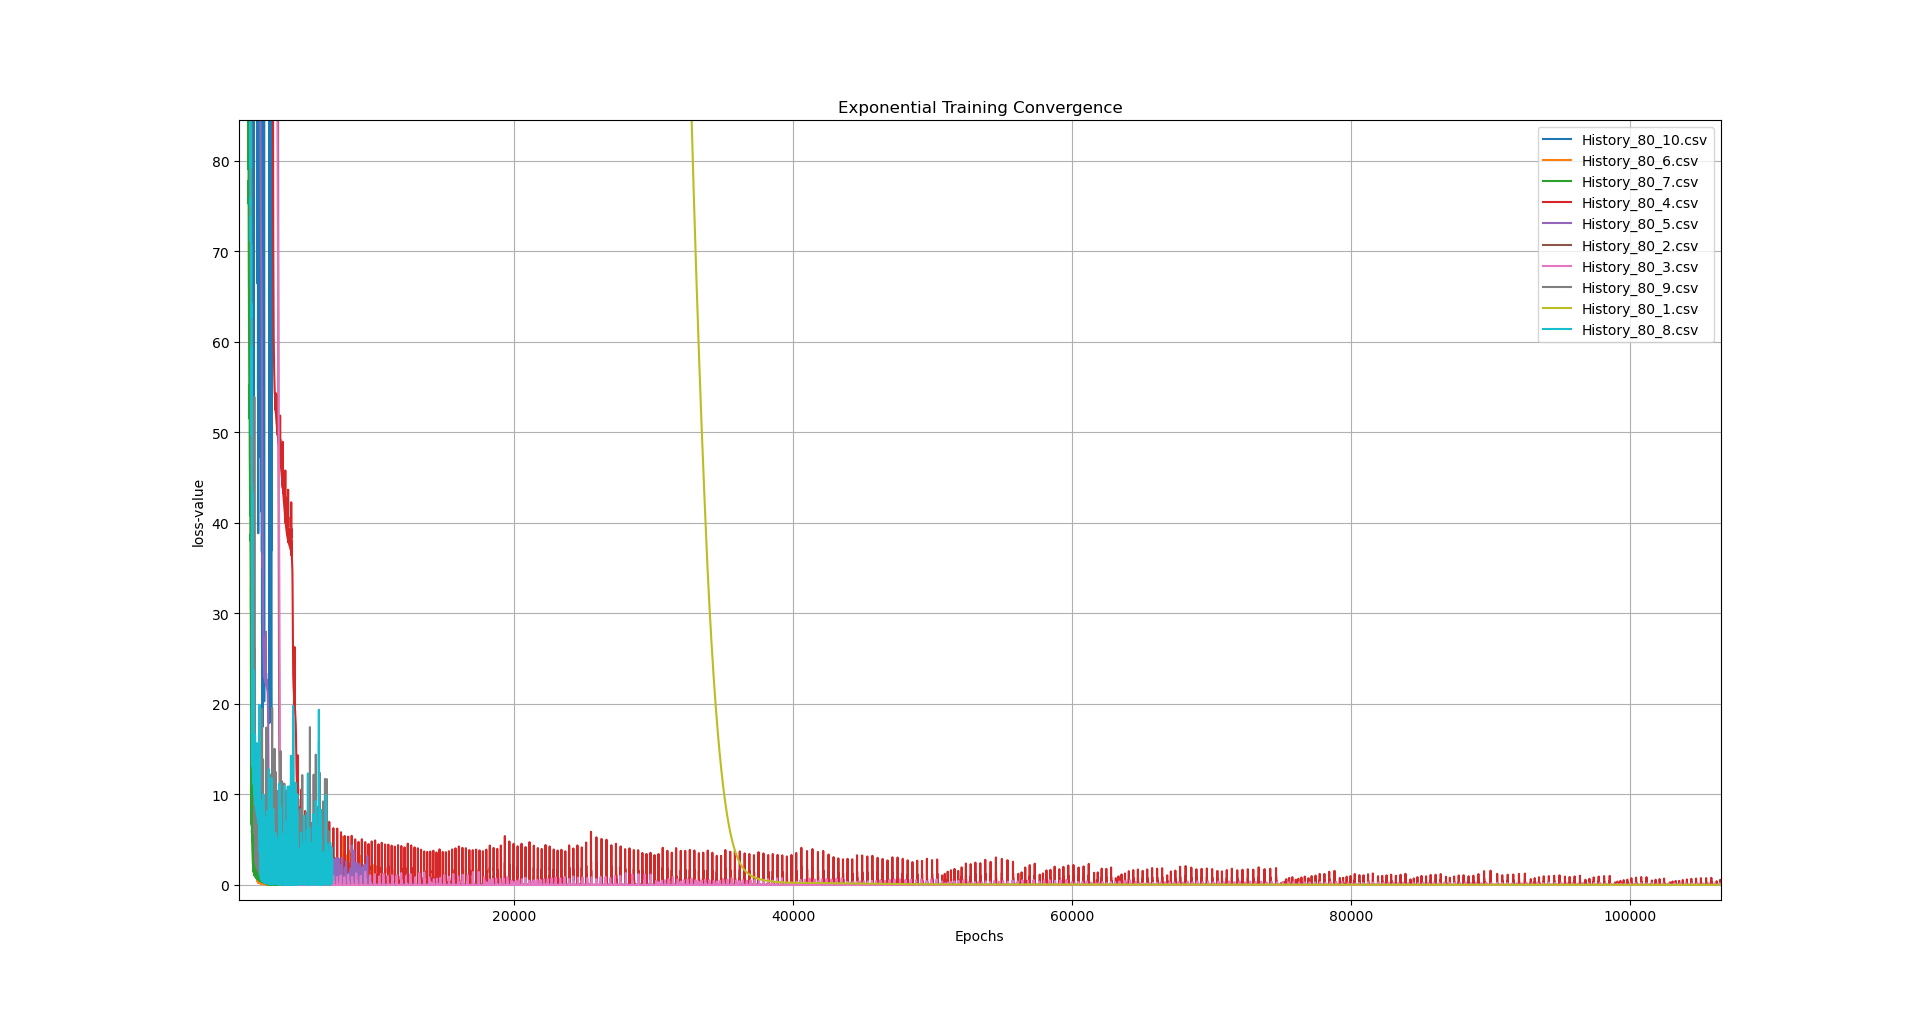
\includegraphics[scale=\size]{Expo_Cons_W.png}
%Seperator
%Seperator
%Seperator
\subsubsection{Plots Across Constant Depth}
\begin{comment}
\end{comment}
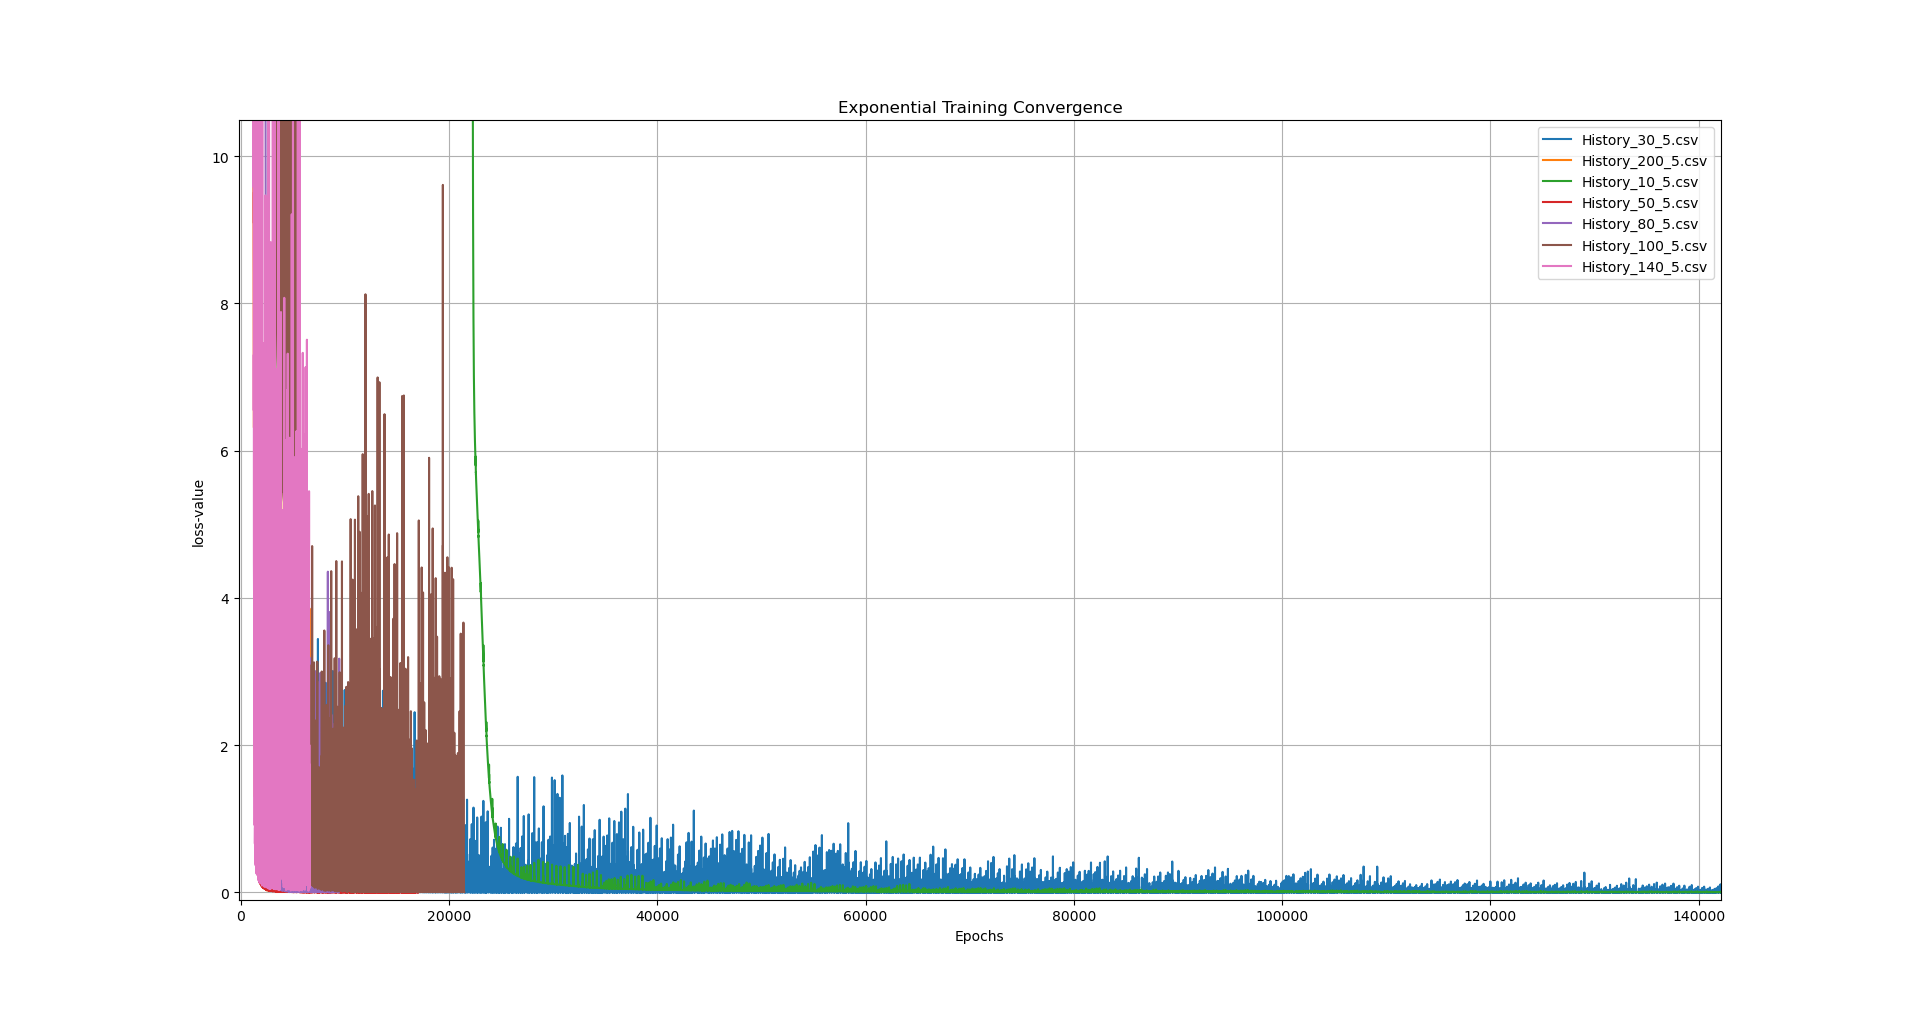
\includegraphics[scale=\size]{Expo_Cons_D.png}
%Seperator
%Seperator
%Seperator
\subsubsection{Comparison to Fixed LR}
\begin{comment}
\end{comment}
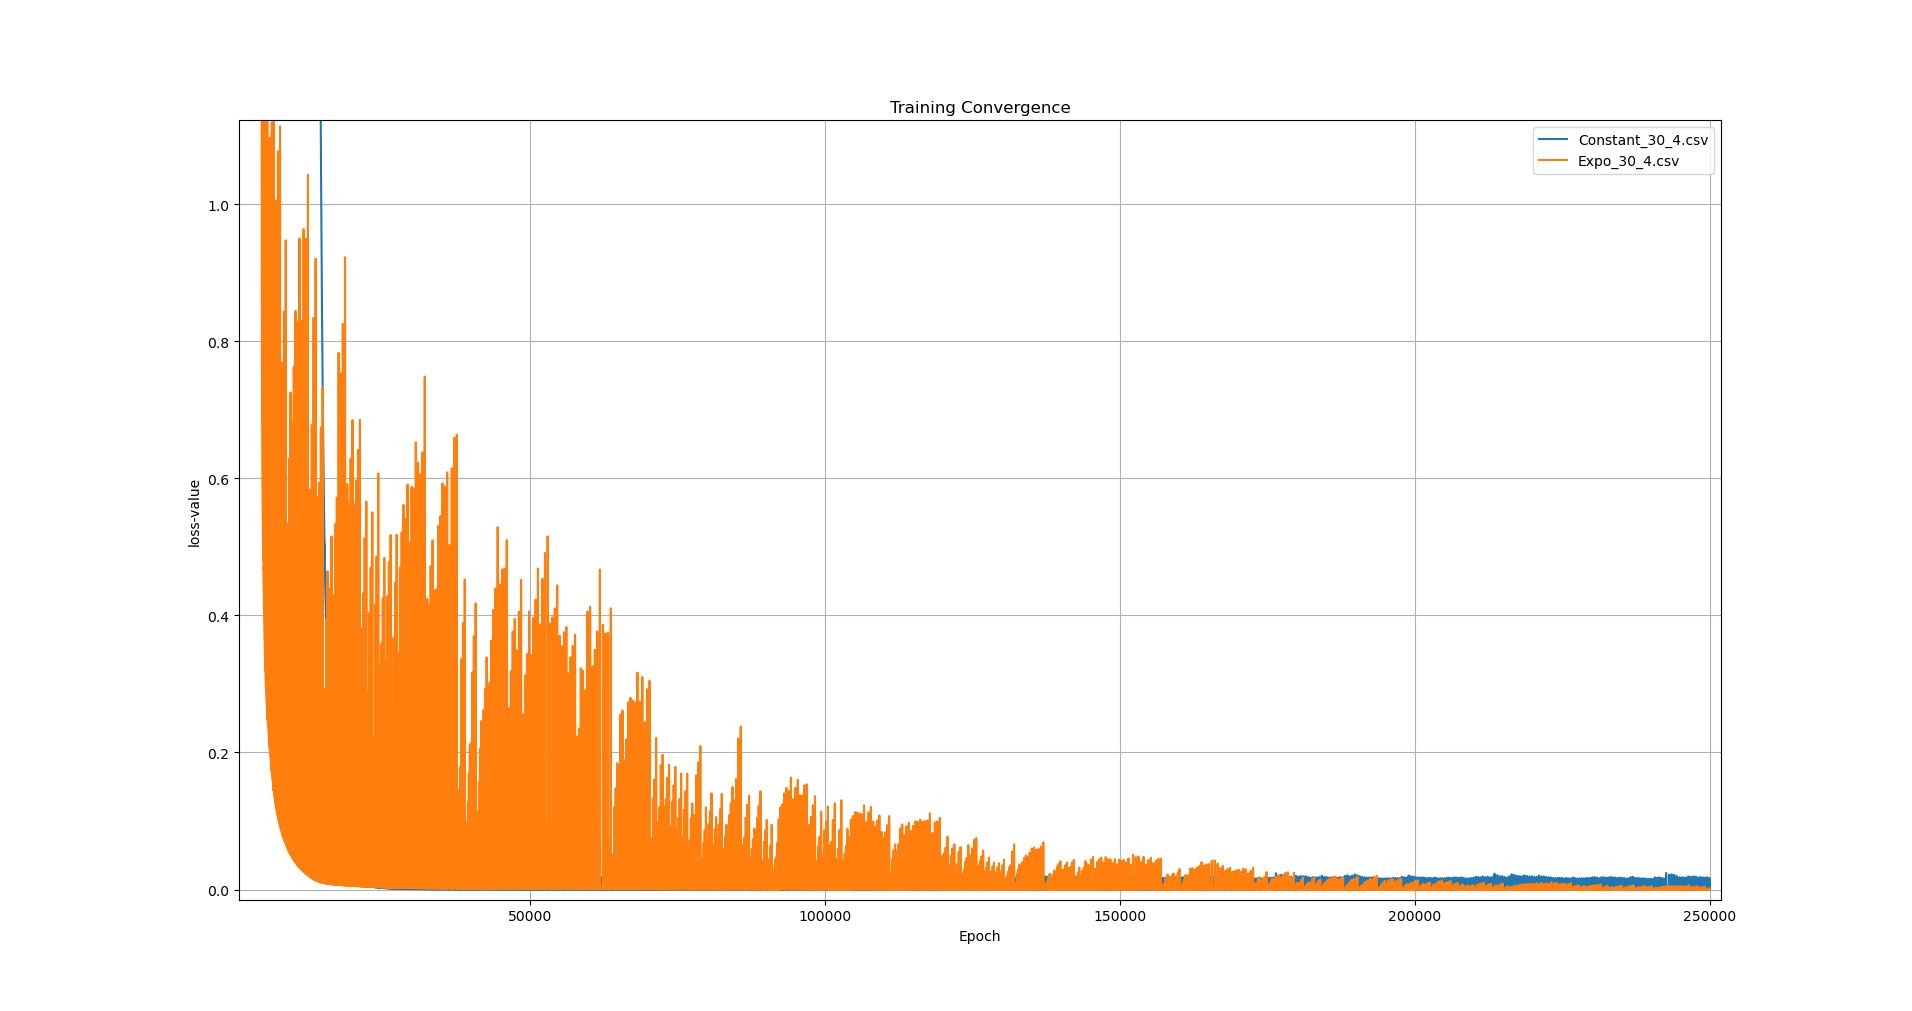
\includegraphics[scale=\size]{Comparison_Expo.png}

%Seperator
%Seperator
%Seperator
%Seperator
\subsection{Polynomial LR}
\begin{comment}
\end{comment}
%Seperator
%Seperator
%Seperator
\subsubsection{Plots Across Constant Width}
\begin{comment}
\end{comment}
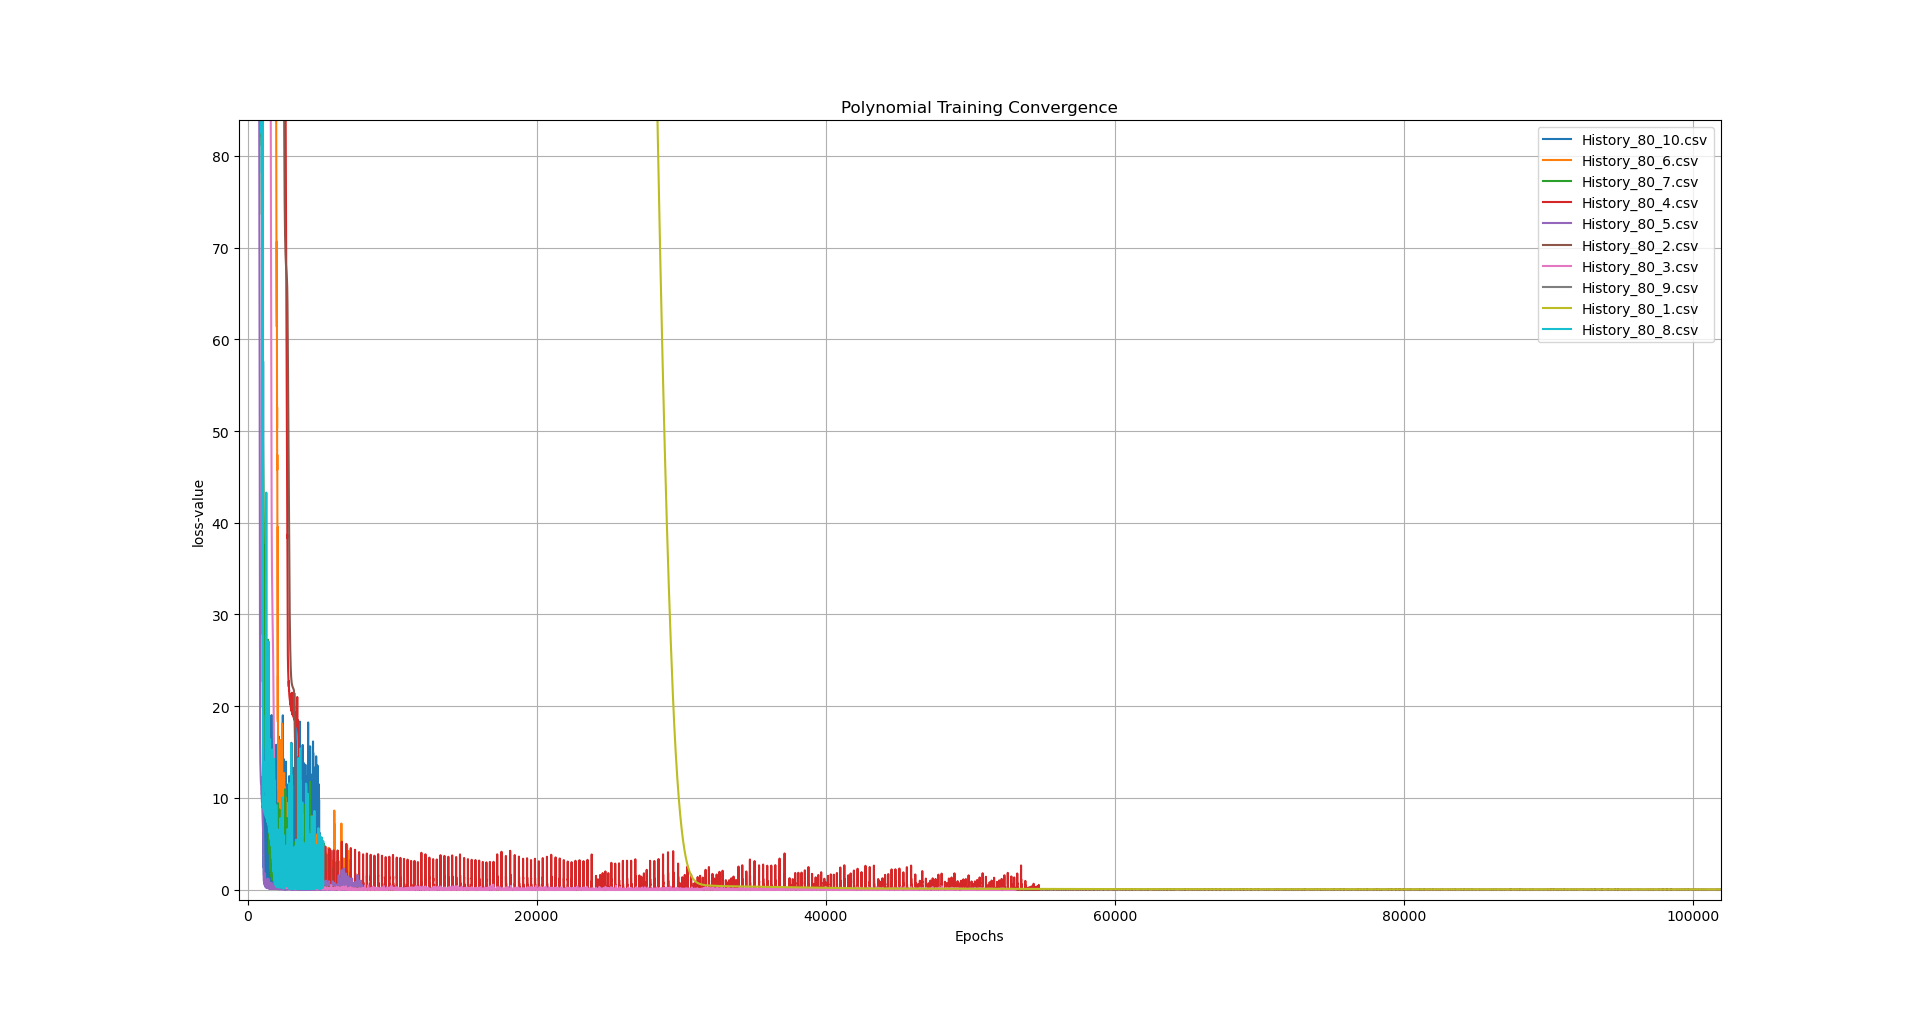
\includegraphics[scale=\size]{Poly_Cons_W.png}
%Seperator
%Seperator
%Seperator
\subsubsection{Plots Across Constant Depth}
\begin{comment}
\end{comment}
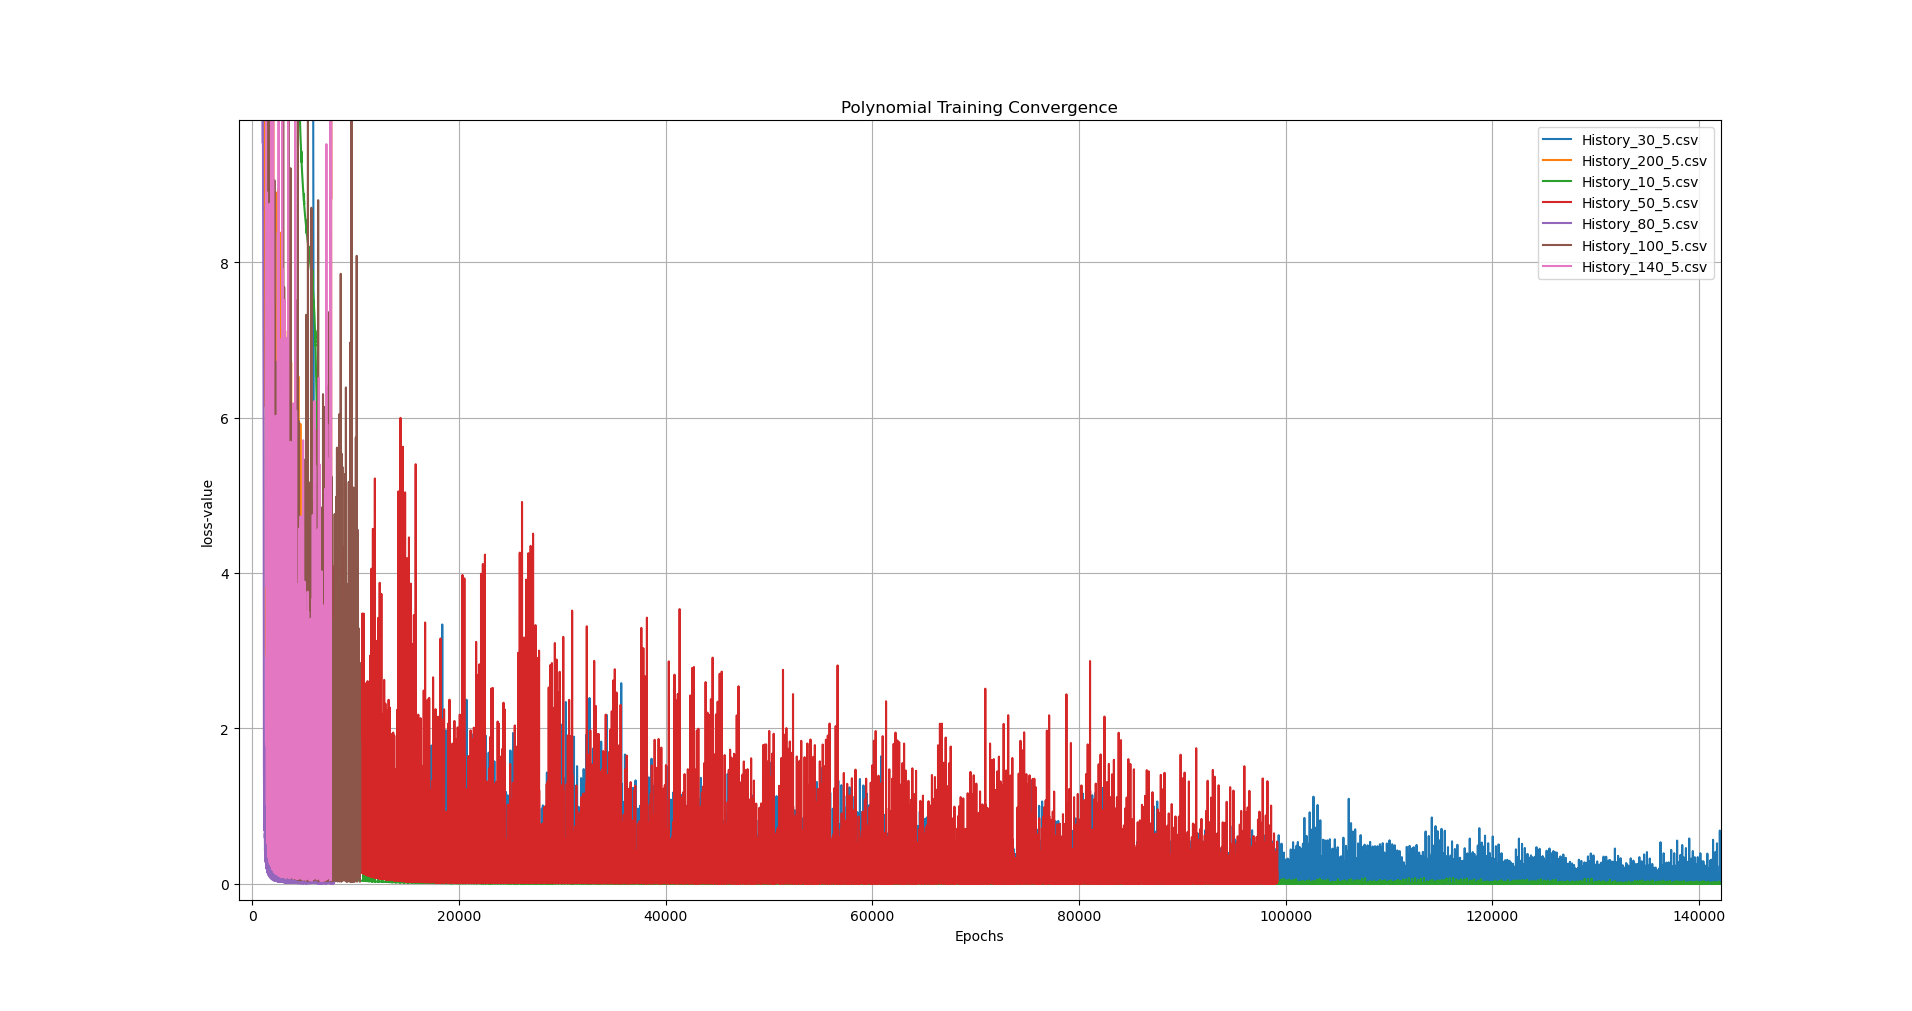
\includegraphics[scale=\size]{Poly_Cons_D.png}
%Seperator
%Seperator
%Seperator
\subsubsection{Comparison to Fixed LR}
\begin{comment}
\end{comment}
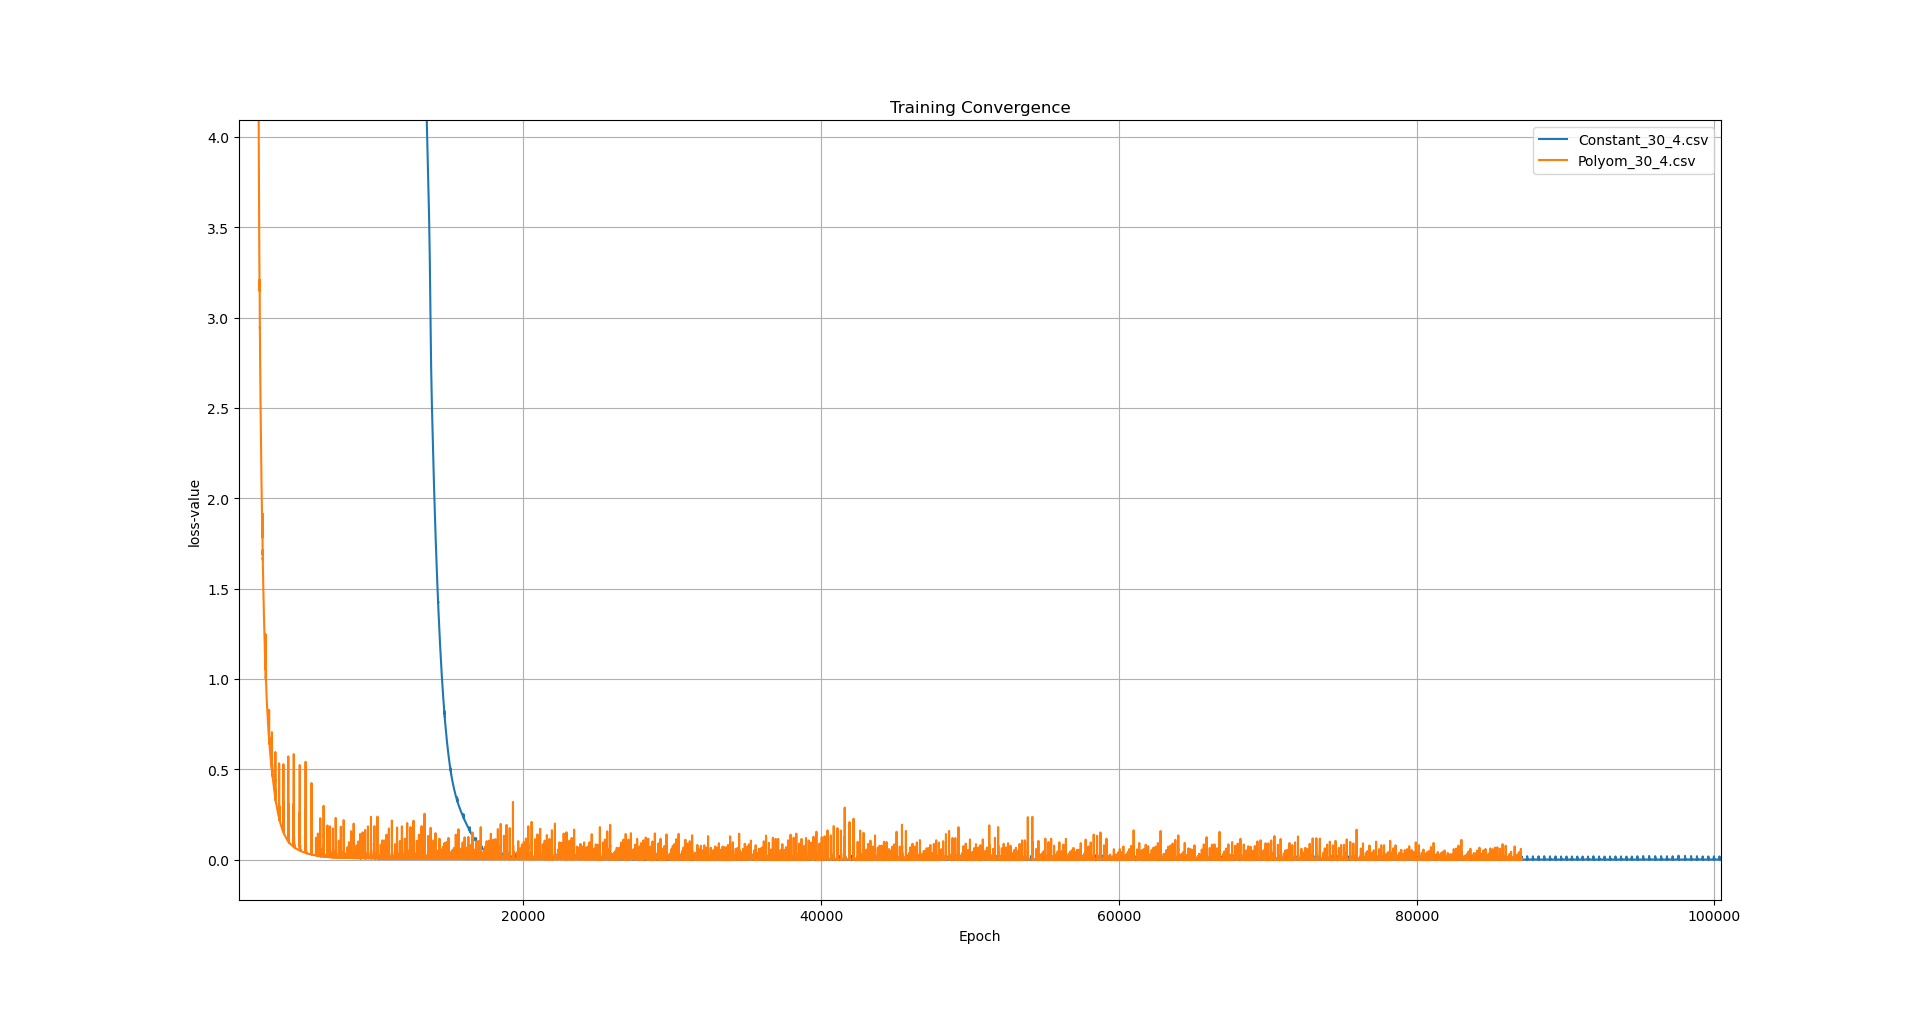
\includegraphics[scale=\size]{Comparison_Poly.png}
%Seperator
%Seperator
%Seperator
%Seperator
\subsection{Inverse LR}
\begin{comment}
\end{comment}
%Seperator
%Seperator
%Seperator
\subsubsection{Plots Across Constant Width}
\begin{comment}
\end{comment}
\includegraphics[scale=\size]{Inv_Cons_w.png}
%Seperator
%Seperator
%Seperator
\subsubsection{Plots Across Constant Depth}
\begin{comment}
\end{comment}
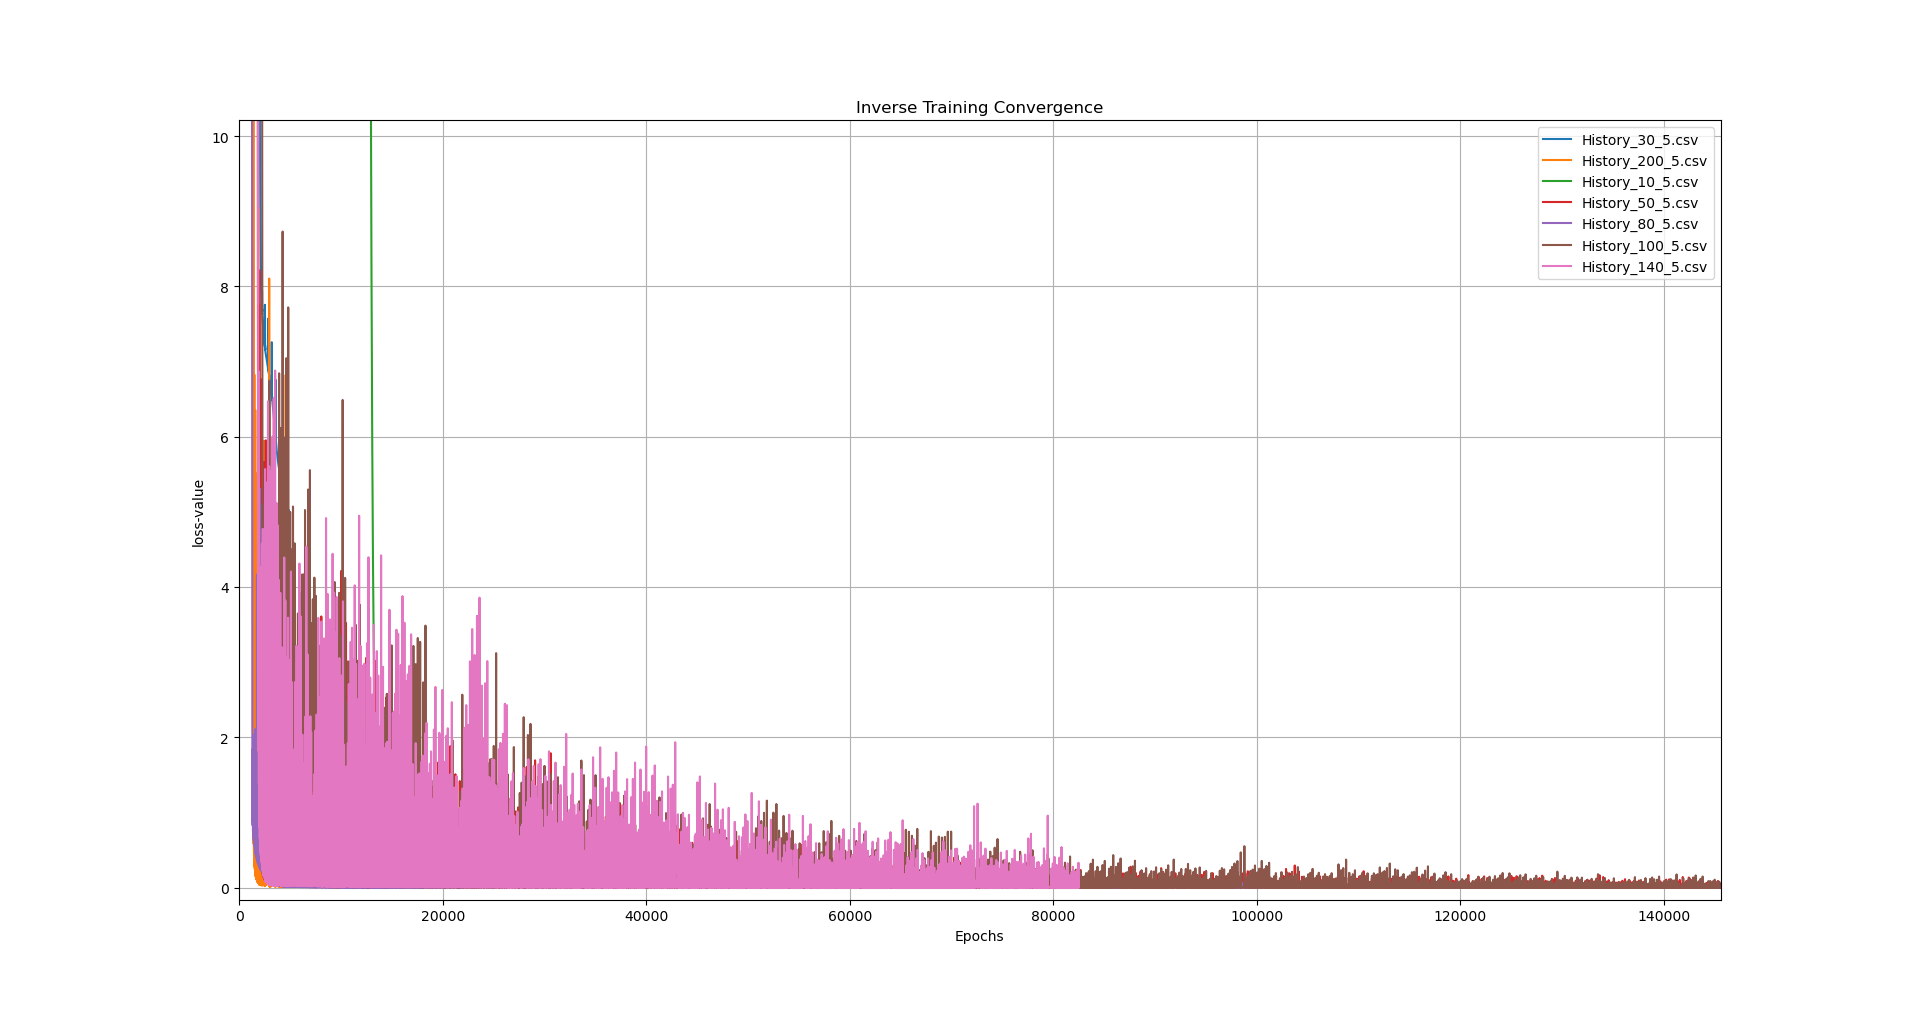
\includegraphics[scale=\size]{Inv_Cons_D.png}
%Seperator
%Seperator
%Seperator
\subsubsection{Comparison to Fixed LR}
\begin{comment}
\end{comment}
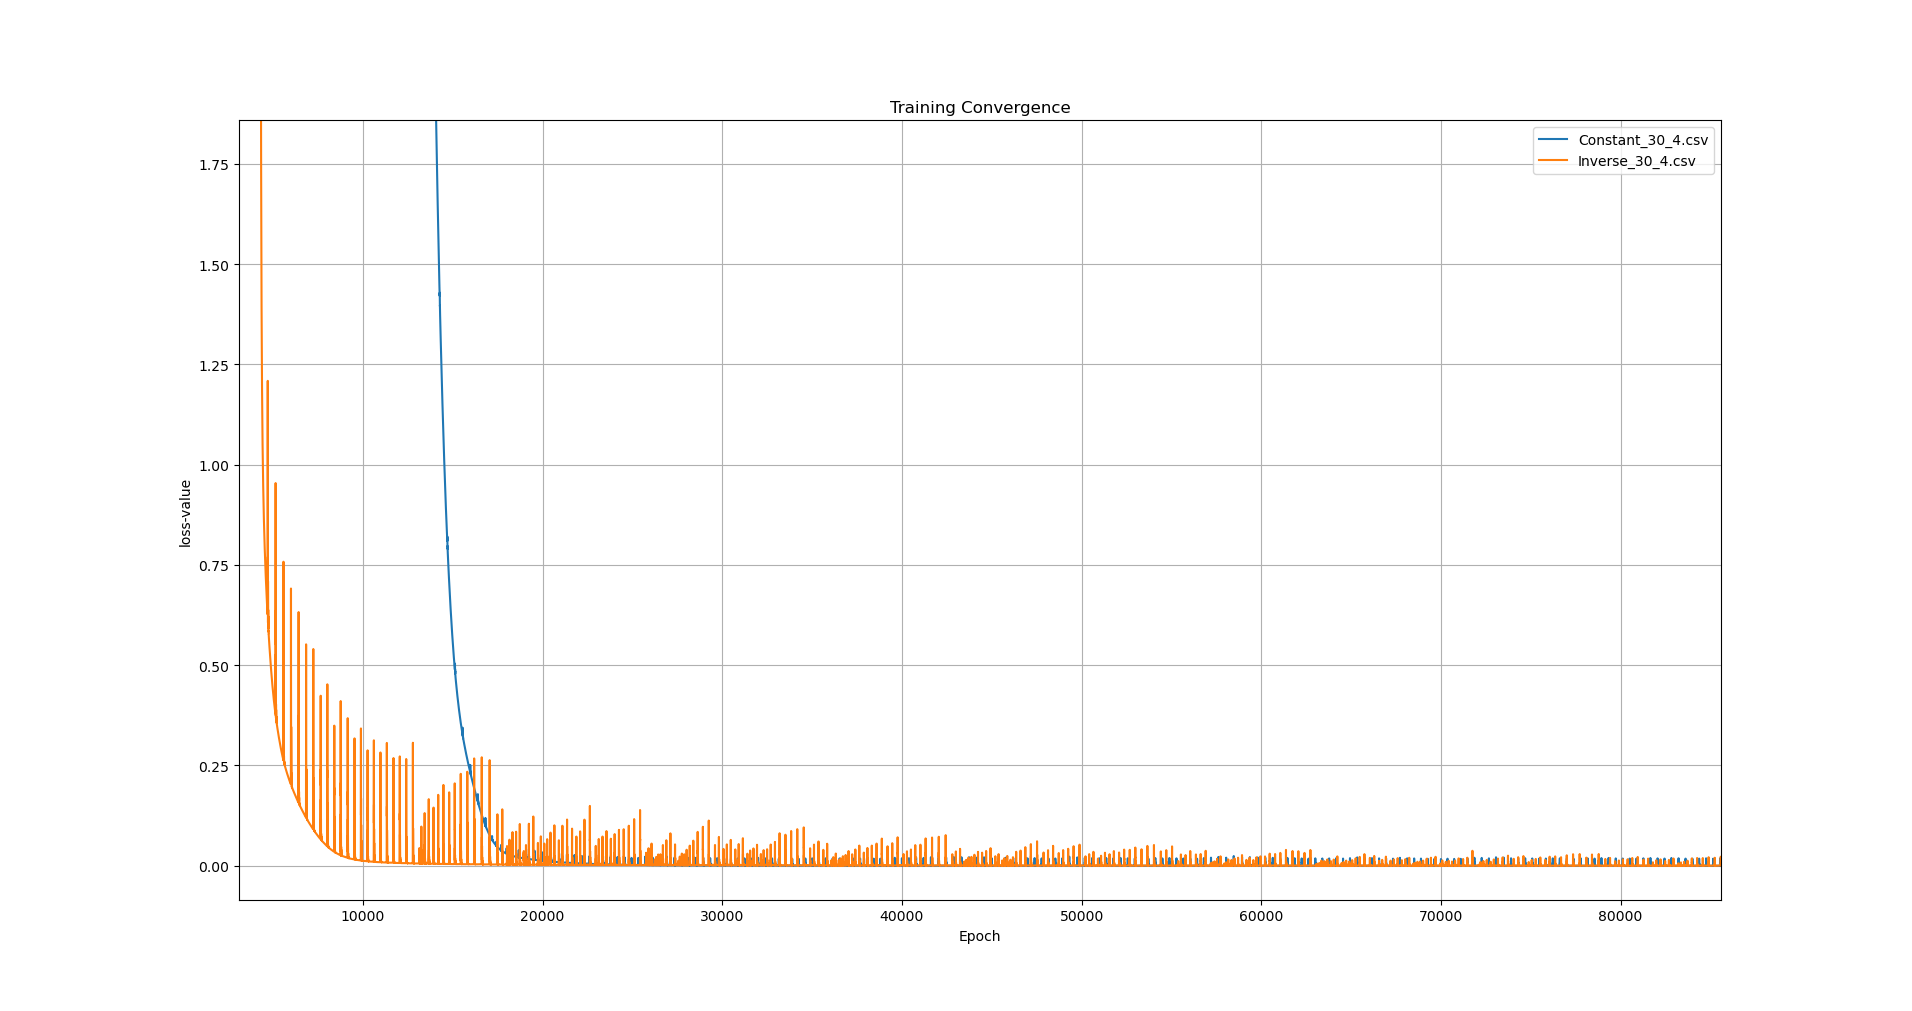
\includegraphics[scale=\size]{Comparison_Inverse.png}
%Seperator
%Seperator
%Seperator
%Seperator
%Seperator
\section{Analysis}
\begin{comment}
\end{comment}
Broadly speaking, having the learning rate scheduler set-up to have a higher initial learning rate and decay to a smaller value improves the training covergence while simulatenously reduces stability issues for some of the scheduler. From observing the plots, it seems that the inverse scheduler is the most stable, followed by the exponential scheduler and finally followed by the polynomial scheduler. The polynomial scheduler has an order $n = 1$. Therefore, the polynomial scheduler is a linar function. The results can be explained well, a scheduler that "more quickly" reduces the scheduling rate is numerically more stable compared to an algorithm that didn't.
%Seperator
%Seperator
%Seperator
%Seperator
%Seperator
\section{Further Development}
\begin{comment}
\end{comment}
This investigation establishes the relationship between learning rate, stability, and trainig convergence. Since the governing equation used may change, it is more useful not to make learning rate dependent on training iterations but instead have learning rate dependent on the magnitude of the weight gradients.
\\~\\More investigations need to be conducted in the numerical instability of the algorithm. It seems that the numerical instability is periodic. Why is this the case? 
%Seperator
%Seperator
%Seperator
%Seperator
%Seperator
\end{center}

\end{document}
